% !TEX TS–program = pdflatexmk
% do not put extra blank pages after each part of the front matter
\documentclass[oneside]{book}

% math formulae
\usepackage{amsmath}
% author affiliation
\usepackage{authblk}
% bibliography
\usepackage[backend=biber,maxcitenames=1,sorting=nyt,style=authoryear]{biblatex}
\usepackage{caption}
% numbering of figures and tables
\usepackage{chngcntr}
\usepackage{csquotes}
% different labels in lists
\usepackage{enumitem}
% interlinear gloss for linguistic examples
\usepackage{expex}
% displaying Polish special characters
\usepackage[T1]{fontenc}
% displaying figures
\usepackage{graphicx}
% links and references
\usepackage{hyperref}
\usepackage{soul}
% this should be the last imported package
\usepackage{glossaries}
\graphicspath{ {figures/} }
% ignore notes in the bibliography
\AtEveryBibitem{
  \clearfield{note}
}
\addbibresource{lit.bib}
% continuous numbering for figures throughout the thesis
\counterwithout{figure}{chapter}
% continuous numbering for tables throughout the thesis
\counterwithout{table}{chapter}
% minimize whitespace on the right side of linguistic glosses; no indentation
\lingset{glrightskip=0pt minus \hsize,glhangindent=0em,extraglskip=-.5ex,aboveexskip=-8pt,belowexskip=-12pt}
% show sections and subsections in the table of contents
\setcounter{tocdepth}{2}
\makeglossaries
% allow inclusion of PDF figures with versions higher than 1.5
\pdfminorversion=6
\newglossaryentry{CVS}{name=CVS, description={continuous vector space}}
\newglossaryentry{DSM}{name=DSM, description={distributional semantic model}}
\newglossaryentry{LOD}{name=LOD, description={Linked Open Data}}
\newglossaryentry{PMI}{name=PMI, description={Pointwise Mutual Information}}
\newglossaryentry{POS}{name=POS, description={part of speech}}
\newglossaryentry{TTR}{name=TTR, description={type-token ratio}}
\newglossaryentry{WSD}{name=WSD, description={word sense disambiguation}}
\newglossaryentry{WSI}{name=WSI, description={word sense induction}}

\begin{document}
\frontmatter
\title{ASRAEL - Acquisition of Semantic RelAtions bEtween Latin nouns}
\author{Konstantin Schulz}
\affil{Humboldt-Universität zu Berlin}
\maketitle
\tableofcontents
\listoffigures
\listoftables
\printglossaries

\chapter*{abstract}
XXXabstractXXX
\mainmatter
\chapter{Introduction}
This dissertation deals with different ways of detecting semantic relations in text corpora. Its focus is more on methodology than on analytical results. Some important restrictions are necessitated by the precise research question: In a corpus of Latin texts, how can we automatically extract semantic relations that are relevant for language learning? I will concentrate only on a subset of the existing phenomena, namely hypernymy and hyponymy. This selection is motivated by the objective of utilizing the obtained insights as the basis for exercises in the process of learning historical languages. Thus, the detection of said relations is not an end in itself, but is to be viewed in the context of how humans learn languages. 

\section{Semantic relations in language learning}
Specifically, recent studies suggest that an improved integration of hyponymy into the learning process can lead to a higher level of language skills \parencite[196]{taslimExperimentalStudyTeaching2014}. Roughly the same procedure is applicable also in the context of artificial intelligence, which highlights the general importance of semantic relations in any kind of language learning effort \parencite[1306]{carlsonArchitectureNeverendingLanguage2010}. The automated extraction of semantic relations from texts can be used for constructing ontologies in specific domains, which is important for language learning because many textbooks are heavily structured according to a range different topics \parencite[192f.]{punuruLearningNontaxonomicalSemantic2012}. 

Since there is a parallel between semantic relations (or ontologies in general) and the way that humans think, it seems reasonable to exploit that connection for learning purposes. This is particularly important for advanced learners' lexical acquisition \parencite[56]{crossleyDevelopmentSemanticRelations2010}. Now, one might be tempted to conclude that predefined lists of basic vocabulary and more advanced semantic relations would be a sufficient help to language teachers. However, static materials und human supervision will probably fail to account for the entire processual complexity of lexical acquisition \parencite[71]{crossleyDevelopmentSemanticRelations2010}. The involvement of artificial intelligence in the modeling of human knowledge about vocabulary faces various problems, including the progression of learning over time \parencite[70]{crossleyDevelopmentSemanticRelations2010}. 

In language learning contexts, this problem extends also to the morphological domain, where it can prove difficult for students to exploit their knowledge about affixation for the acquisition of semantic relations \parencite[248]{gardnerValidatingConstructWord2007}. However, "inflected and derived forms" are exactly what we encounter in the curricular targets for Latin courses, i.e. literary texts. Most textbooks take care of the problem by using hand-crafted Latin texts instead of authentic ones. This leads to a highly problematic transition from textbook to literature, which is already famous among German teachers of Latin \parencite[115]{schibelZurAneignungLateinischer2013}. The challenge, then, is to not only extract semantic relations from a given corpus, but also to group them according to general principles of progression that are tightly coupled with a domain-specific theory of learning.

\chapter{Polysemy}
\section{Word Sense Induction}
\label{polysemyProblemForSemanticRelations}
In order to reach that point, we first need to define the basic object to be acquired, i.e. semantic relations. Unfortunately, this is not a precisely defined research object per se because it strongly depends on our previous knowledge about the possible word senses \parencite[12]{ayseExtractionSemanticWord2011}. Consequently, the sense of a word has to be defined before we can start to learn more abstract representations like hyponymy \parencite[137]{bartunovBreakingSticksAmbiguities2016}. Further obstacles may occur in the case of specific relations like synonymy, where a good operationalization is needed to retrieve the relevant instances from a corpus of text data \parencite[274]{divjakCorpusbasedCognitiveSemantics2009}. In my study, I will focus heavily on the approach of distributional semantics, describing specific semantic relations between words in terms of their co-occurrences, i.e. typical contexts in a corpus \parencites[162]{harrisDistributionalStructure1954}[30]{firthSynopsisLinguisticTheory1957}. This approach has traditionally suffered from several limitations. In some cases (e.g. synonymy), building unified representations for every type in a corpus can prove highly problematic \parencite[114]{karanDistributionalSemanticsApproach2012}. However, this is not universally true anymore as there are \gls{DSM}s that consistently distinguish between various contexts (\hyperlink{ELMO}{see below}). Other problems of distributional semantics are tied to fine-grained distinctions between specific semantic relations \parencite[115]{karanDistributionalSemanticsApproach2012}.

Co-occurrence counts can be a good basis for the detection of semantic relations in general, but they are rarely sufficient for a thorough classification into several subcategories. Nonetheless, previous research has been carried out (more or less successfully) using, e.g., association measures to detect synonymy \parencite[566]{hagiwaraSupervisedSynonymAcquisition2009}. One of the critical parts in that regard is the term `word pair', which introduces the linguistically ill-defined concept of `word' into an otherwise seemingly precise mathematical formula. In the following, we will start by using the term `word' simply as `token in a corpus' and later proceed to a more advanced definition. This progression seems reasonable given the fact that the usage of token-based \gls{PMI} for the research purposes of distributional semantics often leads to severely skewed results \parencite[444]{herbelotMeasuringSemanticContent2013}. Therefore, corpora may have to be tokenized and segmented using more complex separator rules than `whitespace and punctuation' before they can serve as a basis for distributional analyses \parencite[6]{mikolovDistributedRepresentationsWords2013}. Besides, polysemy may also become a problem for resolving other issues like synonymy, e.g. if two words are synonymous only in one of their possibly numerous senses \parencite[444]{herbelotMeasuringSemanticContent2013}. 

In addition to polysemy itself, related concepts like homonymy can also become obstacles with regard to the aim of defining semantic relations precisely \parencite[251]{gardnerValidatingConstructWord2007}. Distributional semantics provides a valuable framework to break down the multiple aspects of meaning for homonymous or polysemous words into smaller subsets, based on the combination with, e.g., adjectival modifiers \parencite[42]{boledaIntensionalityWasOnly2013}. Therefore, the integration of specific contextual elements into the analysis of hyponymy between Latin nouns seems to be a reasonable basis for distinguishing subtle semantic nuances more consistently. As a consequence, polysemy will be treated in this study not just as one of the analytical targets, but also as a methodological aspect that needs to be addressed before other kinds of analyses can be performed. A useful operationalization of polysemy in a distributional context is to look at the collocational diversity \parencite[8]{hamiltonDiachronicWordEmbeddings2016}. This approach brings along the problem of sampling, which is a general one for the whole of corpus linguistics: If we want to model a specific language like Latin as a whole but only use a tiny subset of the available language data for our corpus, how can we expect our results to be applicable to other Latin texts? The key point here is the purpose: For this study, our ultimate goal is not to model Latin nouns per se, but only with regard to the rather well-defined application context of language learning. Therefore, the explanatory power of our linguistic model does not need to be as comprehensive, and it will be restricted to predefined parameters. These parameters may in turn be described as, e.g., the objective of maximizing a student's learning success by providing structured information about semantic relations.

%TODO: add chapter on the choice of PROIEL as corpus... why not AGLDT or ITTB?

\section{Distributional Semantic Models for Word Senses}
Historically, linguistic features of words have often been represented in \gls{CVS}s \parencites{mikolovEfficientEstimationWord2013}{daiDocumentEmbeddingParagraph2015}{akbikContextualStringEmbeddings2018} that can be seen as statistical models of word distributions in natural language \parencite[1140]{bengioNeuralProbabilisticLanguage2003}. Such models map single elements of an utterance (e.g. characters, tokens, types, phrases etc.) to vectors in an n-dimensional \gls{CVS}. Depending on the dimensionality, various kinds of information will be integrated into the model. For instance, lexically related words (e.g. \textit{amor} `love' in PROIEL 86055.22\footnote{For details on the PROIEL corpus, see \textcite{haugCreatingParallelTreebank2008}. Note that, in this study, we only consider the Latin part of the corpus. Dot-separated unique identifiers will be used to refer to segments and tokens in the PROIEL corpus. This is often more precise than the conventional citation model for ancient works (in this case: Cic. off. 1.12) and does not require knowledge about abbreviations of author names or work titles. On the downside, it is corpus-specific and does not offer immediate information about author, work and structural position of the text passage.} and \textit{amare} `to love' in PROIEL 86334.11) usually correspond to vectors whose distance in the \gls{CVS} is rather small. Since most of these models try to predict words in a corpus given their surrounding context \parencite[5]{mikolovEfficientEstimationWord2013}, those words that co-occur frequently will also be mapped to similar vectors in the \gls{CVS}. This basic interaction helps us to distinguish multiple senses of a polysemous word empirically: If each word sense is associated with different contexts and, thus, different co-occurring words, its calculated vector will be different from those of other word senses. Therefore, a very simple evaluation for \gls{DSM}s with regard to \gls{WSI} looks like this:
\begin{itemize}
	\item Given a pair of contexts that
	\item both contain the same word,
	\item classify whether that target word is used in the same sense or not.
\end{itemize}
Formalizing this into a dataset structure, we may provide a plain text file where each each line contains one example for classification. Since Latin is a highly inflectional language, morphological features of the targeted word can differ a lot. Therefore, the actual word forms have to be indicated separately for each context in the example. If they occur multiple times in a context, the dataset should specify which occurrence of the word is to be evaluated. Finally, a binary value (such as `0 / 1' or `true / false') indicates the ground truth for this classification example, i.e. whether the word senses are the same or not. This is the most critical part: `Ground truth' is a dangerous assumption for linguistic phenomena because it suggests a consistent, unchanging goal to be achieved \parencite[129]{leeGeneratingGroundTruth2012}. This desire stems from the formalization that is deemed necessary to systematically evaluate computational language models \parencite[4]{fischerGroundTruthCreation2010}. Usually, such gold standards depend on human expertise, i.e. people that are highly acquainted with the target domain \parencite[519]{uzunerCommunityAnnotationExperiment2010}. In the case of historical languages like Latin, where specialized software and datasets are scarce \parencites[168]{karakantaNeuralMachineTranslation2018}[3]{mcgillivrayMethodsLatinComputational2013}, researchers often have to resort to digitizing analog resources or creating entirely new ones. This kind of curation process can and should rely on successful patterns from datasets for modern languages. Thus, it is reasonable to have a short look at existing comparable resources for evaluation.

The SemCor \parencite{mihalceaSemCorCorpus2008} and MASC-News \parencite[4218]{moroAnnotatingMASCCorpus2014} datasets are \gls{POS}-tagged English corpora where word senses have been annotated using WordNet \parencite{tengiDesignImplementationWordNet1998}. In that sense, such data is both empirical (because it contains authentic historical utterances) and intuition-based (because it uses an external knowledge base for defining the word senses, \hyperref[WordNet]{see below}). There have been attempts to unify \parencite[216]{navigliBabelNetBuildingVery2010} the various knowledge bases that researchers employed to annotate word senses. Promising results were achieved by discussing discrepancies in the face of text corpora, i.e. actual text passages from authentic sources \parencite[127]{bakerWordNetFrameNetComplementary2009}. This development highlights the importance of usage-based linguistics and points towards the need for a more rigorous, bottom-up formalization of word senses. Further approaches to creating datasets for \gls{WSD} include the usage of dictionaries (other than WordNet) as lexical resources \parencites[25]{mihalceaSenseval3EnglishLexical2004}[2]{jimeno-yepesExploitingMeSHIndexing2011}[6]{yuanSemisupervisedWordSense2016} and the usage of glosses as representations of word senses \parencite[8]{luoIncorporatingGlossesNeural2018}. In contrast, \gls{WSI} usually does not rely on external sense inventories, but tries to infer word senses in an unsupervised, empirical manner only from the text itself. State-of-the-art models cluster distributions of vector representations for possible context-dependent substitutes of a word and, thus, are able to detect distinctions between word senses that had not previously been considered in intuition-based sense inventories \parencite[1-4]{amramiBetterSubstitutionbasedWord2019}. Predecessors to this approach directly used a word's surrounding context to construct sense representations for clustering and identified substantial quality criteria for the evaluation of \gls{WSI} models \parencite[876-878]{huangImprovingWordRepresentations2012}:
\begin{itemize}
	\item human judgment on word sense similarity
	\item variation in patterns of meaning (homonymy, polysemy etc.)
	\item variation in parts of speech (esp. nouns, verbs, adjectives)
\end{itemize}
We can certainly add that, in addition to variation, balancing is a decisive factor for the training data \parencites[620]{liuCombiningIntegratedSampling2011}[9]{weiRoleBalancedTraining2013}[1127]{boneApplyingMachineLearning2015}: If we are interested in rare linguistic phenomena, such as subtle semantic differences between almost synonymous words, we need to make sure that they are represented frequently in our training data. The third criterion is most controversial: On the one hand, powerful \gls{WSI} models need to be general enough to provide sufficient results under different circumstances, e.g. in varying domains and registers. On the other hand, modeling word senses for different parts of speech needs to take into account the diverse influences of lexis and syntax: In some settings, nouns may be represented as sets of their hyponyms \parencite[640]{lewisCompositionalHyponymyPositive2019}, while transitive verbs can be modeled as triples together with their arguments, e.g. subjects and objects \parencite[9]{grefenstetteExperimentalSupportCategorical2011}. Such different approaches uncover the intricate nature of formalizing fine-grained semantic distinctions from a distributional perspective. As a consequence, our goal of detecting hyponyms for language learning seems to warrant a modular operationalization with regard to parts of speech. 

\chapter{Nouns}
Our choice of nouns as the target for hyponymy detection is motivated by evidence from language learning. It suggests that nouns are usually easier to acquire, especially in most modern languages, where this class of words is particularly important in everyday language use \parencite[9]{garcia-gamezLearningNounsVerbs2019}. This is relevant for our research because, nowadays, many learners of Latin have acquired as L1 one of the `noun-dependent' languages, e.g. German or French \parencite[51-52]{baidakKeyDataTeaching2017}. Therefore, it makes sense to build on their individual preconditions and focus, at least initially, on those word classes that are also important in their L1. However, Latin has often been described as verb-heavy language \parencite[41]{mengeLehrbuchLateinischenSyntax2009}. This claim is supported by comparing the noun-to-verb ratio \parencite[300]{stollNounsVerbsChintang2012} of the PROIEL corpus to the Hamburg Dependency Treebank \parencite{borgesvolkerHDTUDVeryLarge2019} and the French Treebank (\cite{seddahCheatingParserDeath2018}; see Table \ref{tableNounToVerbRatio}).
\begin{table}[ht]
	\begin{tabular}{ c | c | c | c }
  		 & PROIEL & French Treebank & Hamburg Dependency Treebank \\ \hline
  		Noun-to-Verb Ratio & 0.50 & 0.71 & 0.73 \\
	\end{tabular}
	\caption{Noun-to-verb ratio for different treebanks in the Universal Dependencies corpus (Latin, French, German; \cite{nivreUniversalDependenciesV12016}).}
	\label{tableNounToVerbRatio}
\end{table}

The lower ratio indicates that Latin authors use fewer nouns, relative to their usage of verbs and compared to authors of modern European languages. This typological difference seems to demand a stronger focus on verbs instead of nouns, at least for Latin. Nonetheless, it has been shown that nouns play a substantial role in the early stages of language acquisition, especially in the understanding of subcategorization frames for verbs \parencite[1383]{yuanCountingNounsSimple2012}. If this is applicable to historical languages as well, we should rather rely on finding suitable combinations, provided that there is a useful formalization of hyponymy for the different parts of speech. The focus on a single word class (in our case: nouns) is one initial step in that direction.

\chapter{Hyponymy}
After dealing with various issues of polysemy, some of the second-tier semantic relations may have to be redefined when looked at from a distributional perspective, e.g. hyponymy \parencite[443]{herbelotMeasuringSemanticContent2013}. In this view, other existing taxonomies that may have acted as models of hyponymy need to be replaced by a definition that reflects how actual usage contexts can limit our selection of possible candidates for hyponymy \parencite[443]{rollerInclusiveSelectiveSupervised2014}. Unfortunately, this view may clash with the observations of \textcite{herbelotMeasuringSemanticContent2013}:
\begin{itemize}
      \item Hypernyms can have very specific usage contexts.
      \item Collocations may lead to unexpected results in the distribution of words.
\end{itemize}
Similar adjustments have to be made in treating other kinds of semantic relations. Therefore, many researchers apply preprocessing to their corpora before performing the actual analysis on them \parencite[56f.]{gyllenstenRgramsUnsupervisedLearning2019}. However, this increases the danger of circularity, revealing only those results that we were already expecting in the first place. As an alternative, we should look for a model that is robust enough to detect semantic relations despite the confounding factors. The objective should be to fit the model to the base text, not the other way round. For vector space models like Skip-gram \parencite[5]{mikolovEfficientEstimationWord2013}, subsampling and the restriction of strong collocations may be justified from a computational perspective because they enable a faster training of models while more or less preserving the resulting performance in the prediction of word contexts. This very tradeoff, though, may not work out as well for the detection of semantic relations, e.g. if we give a higher priority to the frequency of certain contexts. Such a change of algorithm may particularly be motivated by the distinction of theoretical and empirical scopes of words \parencite[46]{coenenAnalogieUndMetapher2013}. 

\label{distributionalInclusionHypothesis}
This also applies to the domains of corpus linguistics and language learning: Given a text corpus that helps learners to acquire a certain knowledge (e.g. all the ancient literature mentioned in an educational curriculum for the Classics), the theoretical scope of a certain word would be equivalent to the set of all distinct contexts in the corpus in which that word occurs. In contrast, the empirical scope of that same word would be equal to a subset of that theoretical scope, namely those contexts which are already known to the learner (at any given point in time of the learning process). Thus, the theoretical scope will remain static as long as we do not change the corpus, while the empirical one will be dynamic as long as we keep learning. From this point of view, we can also restrict our notion of semantic relations: Hyponymy, for instance, will be tied to those lexical networks that are present in a specific corpus and, for a specific learner, specific instances of hyponomy relations will not exist unless they have already been encountered in the corpus and lead to a relevant learning process. It is therefore our duty to a) detect such instances in the corpus and b) use them to design learning situations that help language learners to construct lexical and semantic knowledge \parencite[25]{yorkConstructivistApproachGamebased2018}. In order to accomplish that first part, we need to have clearly defined requirements to qualify a relation as one of hyponymy, e.g. according to a version of the Distributional Inclusion Hypothesis \parencite[443]{rollerInclusiveSelectiveSupervised2014} that also accounts for idiomaticity, burstiness and other kinds of lexical interferences.

\section{WordNet}
\label{WordNet}
Lexical resources like the Latin WordNet \parencite{minozziLatinWordNetProject2010} may contribute a reference model for such a purpose because it includes a built-in notion of hyponymy. Unfortunately, the WordNet defines such relations based on intuition, not on actual language use \parencite[315]{fellbaumChallengesMultilingualWordnet2012}. WordNet is therefore static and non-empirical from the perspective of usage-based fields like corpus linguistics. However, it was constructed by alleged experts and we may use their assessment for reflecting our own approach. This kind of triangulation is supported by recent studies, which often explicitly combine knowledge bases and corpus data \parencite[984-988]{onoWordEmbeddingbasedAntonym2015}, thereby integrating both the introspective and the usage-based approaches to semantics. The former can be helpful in two ways: a) by defining a horizon of expectations in language learning contexts, i.e. which information learners are supposed to infer from their previous knowledge in order to understand a linguistic expression in a specific text passage; and b) by modeling semantic knowledge in a machine-readable, consistent (albeit simplistic) manner. The integration of distributional semantics, on the other hand, is particularly motivated by the hypothesis that semantic properties of words are reflected in their contextual surroundings \parencite[59]{griesBehavioralProfilesCorpusbased2009}. 

By using distributional data from corpora, we also gain the advantages of rigorously empirical research (as opposed to bare intuition and anecdotal evidence): frequency, authenticity, variation and systematic induction \parencite[60]{griesBehavioralProfilesCorpusbased2009}. Still, knowledge databases may be useful for languages like Latin where previous research is scarce and, more often than not, heavily intuition-based or anecdotal. In both the introspective and the distributional case, we can increase the amount of provided information by relying on associated properties of hyponymy relations, e.g. transitivity \parencite[58]{coenenAnalogieUndMetapher2013}. Applied to the Latin WordNet, this may look as follows:
\begin{enumerate}
         \item \textit{gladius}
         \item a cutting or thrusting weapon with a long blade
         \item weaponry used in fighting or hunting
         \item weapons considered collectively
         \item an artifact (or system of artifacts) that is instrumental in accomplishing some end
         \item a man-made object
         \item a physical (tangible and visible) entity
\end{enumerate}
This information flow can be read from both sides. Beginning at \textit{gladius} (sword), it can be used to simulate the process of reading a text: We encounter a word in the text (e.g. the plural \textit{gladii}) and determine its lemma (\textit{gladius}). From there, we can try to find a corresponding meaning for the surface form, e.g. "a cutting or thrusting weapon with a long blade". This meaning, in the WordNet taxonomy, can be hyponym to other kinds of meaning, e.g. "weaponry used in fighting or hunting". Now, if we know that
\begin{itemize}
         \item \textit{gladius} is a weapon with a blade and
         \item weapons with a blade can be used for hunting,
\end{itemize}
then we are safe to assume that a \textit{gladius} can be used for hunting. The further we go down the list, the more abstract do the meanings get. Nonetheless (or because of that), every layer can remind us of new specific features that we may want to associate with \textit{gladius}: specific motion (2.), specific purpose (3.), hypernym (4.), general purpose (5.), origin and production (6.), material (7.). In some cases, we may even use morphological hints to get faster access to information about hyponymy \parencite[913]{anstattTypenSemantischerRelationen2009}. This is especially true for Latin with its relatively rich morphology: the meaning of \textit{artifex} (artist) may be associated directly to \textit{ars} (art) and \textit{facere} (to make), without necessarily traversing a hierarchical tree-like representation of increasing semantic generalization. Interestingly, this is possible even in cases where the compound is formed from foreign language material and thus cannot be easily paraphrased in the native language \parencite[33]{souille-rigautSemanticAccountQuasiLexemes2010}. 

How is that important for Latin hyponymy? Consider Greek loanwords: \textit{xylophytum} (a certain kind of plant) cannot be reasonably described in Latin words as a \textit{*phytum} that is made of \textit{*xylum}. However, Romans may have deduced that the meaning of \textit{xylophytum} is related to ($\rightarrow$ hyponymy) \textit{-phyt-}, thereby inferring previous knowledge about plants. Therefore, we have to allow for the possibility that some instances of hyponymy may not be extractable solely on a distributional basis, but rather on a morphological one. Besides, a morphologically informed model is able to explain why we can immediately see semantic structure in newly coined words \parencite[43]{souille-rigautSemanticAccountQuasiLexemes2010}. In this respect, knowledge about specific hyponyms or hyponymy in general can facilitate the language learning process by providing a rather intuitive access to the meaning of single words or phrases. Unfortunately, this intuition sometimes competes with other interpretations of a word's sense which may be equally intuitive and valid \parencite[126]{ponsborderiaPathsGrammaticalizationSpanish2014}. 

Such examples underline the importance of disambiguation (\hyperref[polysemyProblemForSemanticRelations]{see above}), which may not always be possible. Furthermore, additional steps may be necessary even if a specific word sense was already determined, e.g. the inference of common knowledge or common sense \parencite[427f.]{pinkalSemantik1993}. In this view, disambiguation should be preceded by a thorough linguistic analysis of the context, which, in terms of distributional semantics, is usually addressed by extracting cooccurrence frequencies from sliding windows over a textual input, be it plain text or a linguistically annotated treebank. However, the integration of external information into this process is not as straightforward and therefore often avoided. In the end, this might not be the worst decision, depending on our definition of semantics: Some models of distributional semantics reduce the spectrum of polysemy to one main aspect of meaning per word.
\parencite[4]{faruquiProblemsEvaluationWord2016}.

\hypertarget{ELMO}{Approaches} of this kind level nuances that may actually be important for our understanding of a single word in its context. As an improvement, other models regard entire sentences for the representation of a word's context-specific meaning, thereby differentiating between various common usages \parencite[2f.]{petersDeepContextualizedWord2018}. Modeling the process of language production both in a forward and backward manner at the same time seems reasonable, especially for the Latin language, because the antecedent of, e.g., a relative pronoun can be part of the relative clause, which makes it difficult to understand the structure of such a construction by reading it in just one direction, without referring to the past and future context at the same time:\footnote{The glossing of longer Latin text passages was created according to the \href{https://www.eva.mpg.de/lingua/pdf/Glossing-Rules.pdf}{Leipzig Glossing Rules}.}

\vspace{10pt}
\ex[exno=PROIEL 53467]
	\par
	\begingl
		\gla nam et frument-um ex agr-is cotidie in castr-a confere-ba-t et qu-ae grav-issim-e adfli-ct-ae era-nt nav-es e-a-rum materi-a atque ae-re ad reliqu-a-s reficie-nd-a-s ute-bat-ur [...] //
		\glb since also grain-{\sc acc} from field-{\sc abl.pl} daily-{\sc adv} into camp-{\sc acc.pl} convey-{\sc impf-3sg} and which-{\sc f.pl} heavy-{\sc sup-adv} strike-{\sc pass-f.pl} be-{\sc 3pl} ship-{\sc pl} this-{\sc f-pl.gen} timber-{\sc abl} and brass-{\sc abl} to remaining-{\sc f-pl.acc} repair-{\sc gdv-f-pl.acc} use-{\sc impf-3sg}//
		\glft for he daily conveyed corn from the country parts into the camp, used the timber and brass of such ships as were most seriously damaged for repairing the rest [...] //
	\endgl
\xe
\vspace{10pt}

In this example, \textit{naves} is the antecedent to the relative pronoun \textit{quae}. Its integration into the relative clause is recognizable by its morphological congruency (case, number, gender) with the relative pronoun. In a textbook setting, the sentence would rather look like this: \textit{[...] conferebat et earum navium, quae gravissime adflictae erant, materia atque [...]}. Such syntactic variations are probably related to the relatively free word order in the Latin language. Therefore, a language model for Latin should be flexible enough to analyze a given textual sequence by looking at either the left or right context, according to the circumstances of the case \parencite[8]{devlinBERTPretrainingDeep2019}. While this strictly bidirectional, attention-based approach \parencite{vaswaniAttentionAllYou2017} enhances the ability to explain word meanings from their larger surrounding contexts, it does not address the problem of inference, e.g. relevant external text passages. To analyze this problem empirically, we will set up a toy language model in order to inspect difficult cases. 

\chapter{Method}
\section{Experimental Setup}
General notes on the agility and openness of the methods applied in this study can be found in the \hyperref[sec:appendixA]{Appendix A}. Now, it is time to have a closer look at the separate steps in the workflow:
\begin{enumerate}
         \item Create a dataset.
         \begin{enumerate}
		\item Specify the text corpus to be used.
		 \begin{enumerate}
			\item Segment the corpus into smaller pieces, e.g. sentences.
			\item Tokenize every segment.
		\end{enumerate}
		\item Specify a gold standard for hyponymy.
		\item Define hyponymy pairs for every segment in the corpus.
	\end{enumerate}
         \item Split the dataset into subsets for training, validation and evaluation.
         \item Implement a transformer language model \parencite{vaswaniAttentionAllYou2017} for hyponymy extraction.
         \begin{enumerate}
		\item Train the model on the training subset.
		\item Use the validation subset to make sure that the model inferred general rules instead of memorizing input patterns.
	\end{enumerate}
         \item Evaluate the model using the evaluation dataset.
\end{enumerate}
Since machine learning is the major approach to be considered here, the size of the dataset (especially the training subset) is crucial \parencite[13]{hestnessDeepLearningScaling2017}. The rule of maximizing training data applies not only to machine learning, but also to other methods of distributional semantics, e.g. in the case of semantic relations \parencite[27]{herbelotBuildingSharedWorld2015}. Therefore, it seems reasonable to prefer the Corpus Corporum (about 190 million tokens of plain text, cf. \textcite{roelliCorpusCorporumNew2014}) over PROIEL (about 220.000 tokens of annotated text). Unfortunately, this limits the usage of linguistic research results (i.e. annotations) as input for the language models. On the other side, the practical application of the model for language learning purposes becomes easier and more flexible, in the sense that, theoretically, end users can supply any plain Latin text of their choice, without the need to provide additional annotations.

Before we can start to detect hyponyms, we need to induce word senses, especially for polysemous words. To make sure that fine-grained distinctions between different usages of the same word are recognized by the model, it should be evaluated on a test dataset that has the following structure:
\begin{itemize}
	\item For each segment in a pair of segments (e.g. sentences),
	\item look at the target word(s) and
	\item predict whether it was used in the same sense as in the other segment.
\end{itemize}
The second step can be formalized by providing character indices referring to the position of the target word in a string representation of the segment. This works even for cases where a target word form occurs multiple times in the segment and we want to induce the word sense for just a single specific instance. The third step, i.e. prediction of semantic similarity, can be binary in this very basic operationalization: The two target words are either used in the same sense or not. This dichotomy consciously abstracts from more complicated evidence, e.g. where two instances are used in a very similar, but not quite the same sense. In a subsequent effort, we may try to associate the current instance with other segments where the word usage is similar, thus clustering occurrences of the same word sense together. 

Since there are no semantically annotated authentic text corpora for Latin, the next best thing to use are grammar books and dictionaries: They often distinguish between various word senses and offer exemplary contexts for each one \parencites{georgesAusfuhrlichesLateinischDeutschesHandworterbuch1913}{niederauNavigiumLateinDeutschWorterbuch2012}. Some of them cite entire text passages \parencites{shortLatinDictionary1879}{kuhnerAusfuhrlicheGrammatikLateinischen1914}{mengeLehrbuchLateinischenSyntax2009} to support their classifications. Such references can be seen as annotations: If a dictionary lists various text passages as containing a specific word in the same sense, this is roughly equivalent to semantically annotated datasets where sense identifiers from static sense inventories are assigned to tokens in a text corpus. Now, we could proceed by looking at the largest entries in a dictionary, assuming that they contain the largest number of different word senses. This, however, would amount to accepting the dictionary editor's intuition, which is not a usage-based approach. Instead, we will find the most polysemous words in a corpus inductively, by looking at their usage contexts. In this view, the most polysemous word will be that which is used in the most diverse contexts.

A naive formalization of diverse contexts is to count the number of types that occur in the same sentence as a target type in the corpus. This disregards the absolute frequencies of the types in a corpus and will lead to a Zipfian distribution \parencite[VI]{zipfPsychobiologyLanguageIntroduction1936} of target types. Thus, function words like \textit{et, in, ut, est, non, cum} `and, in, as, is, not, with' will dominate the ranking just because of their immense absolute frequency in the corpus. We can limit their impact by randomly down-sampling their occurrences using an arbitrary upper bound of 100.
\label{high_frequency_hyponyms_for_language_learning}
Since our goal is to produce exercises for language learning, the potential hyponyms should be rather frequent in a given corpus \parencites[27]{ellisUsagebasedLanguageInvestigating2013}[2]{robillardMonolingualBilingualChildren2014}. It is therefore reasonable to establish a minimum threshold for word frequency. This criterion interacts with Latin being a highly inflectional language, thus producing many morphologically different forms for the same lexeme (see Table \ref{tableTypesPerLemma}).
\begin{table}[ht]
	\begin{tabular}{ c | c | c | c }
  		 & PROIEL & French Treebank & Hamburg Dependency Treebank \\ \hline
  		Types per Lemma & 3.64 & 1.21 & 2.09 \\
	\end{tabular}
	\caption{Average number of types per lemma for Latin, French and German.}
	\label{tableTypesPerLemma}
\end{table}

%TODO: did we really use lemmatized texts?
Thus, we will perform this initial experiment on professionally lemmatized texts, which restricts us to the PROIEL treebank. Using lemmata instead of types has the advantage of increased frequency counts per item (esp. in small corpora) and allows us to easily group contexts by lexeme. The downside here is that the diversity of contexts cannot be distinguished anymore for various word forms of the same lexeme, but we can reintroduce that distinction in a later step. The comparison of two contexts for a given target word will be made using representations of sentences in a \gls{CVS}. This mapping from textual to numerical entities (i.e. vectors) is not straightforward, because it is unclear how exactly we should model the difference between short and long sentences that share roughly the same content, but with different wording. 

%TODO: add comparison of different vector measures, including Euclidean distance, cosine distance etc.
If we pad all shorter sentences to an arbitrary upper bound (e.g. the length of the longest sentence in the corpus) using placeholder values, the model will be able to calculate the cosine similarity\footnote{Throughout this thesis, the terms \textit{cosine similarity} and \textit{cosine distance} will be used interchangeably. The distance is usually a value between -1 and 1. The similarity is usually calculated by subtracting the distance from 1.} \parencite[3]{luoCosineNormalizationUsing2017} between two sentence vectors as input. However, naively using a fixed value as the placeholder in right-padded sequences \parencite[386]{sachanEffectiveUseBidirectional2018} is equivalent to assuming that, compared to very long sentences, every short sentence tends to repeat the same word over and over again after a certain time. From a linguistic perspective, this formalization seems rather unintuitive because it does not take into account the effects of text length on lexis \parencites[31]{golcherStylometryInterplayTopic2011}[141]{ochabStylometryLiteraryPapyri2019}, which may lead to a clustering of input sentences roughly by (original) sequence length.

\section{Sensitivity to Lexical and Syntactic Variation}
%TODO: describe the transformer model (layers, parameters etc.)
%TODO: explain why positional encoding is important in Latin, even for distributional semantics
Against this backdrop, normalization of text length is probably just as problematic as the disruptive influence of text length in the first place. Possible alternatives consist in manual ad hoc annotation or trying to circumvent the problem. We will proceed by testing a model of semantic diversity that includes lexical and syntactic cues while also ignoring text length. By training a transformer language model \parencite[9]{vaswaniAttentionAllYou2017} on the raw text of the PROIEL corpus, we build a \gls{CVS} into which single tokens can be embedded. Our implementation uses Positional Encoding \parencite[4]{conneauCrosslingualLanguageModel2019} to explicitly analyze every word's position in a given sequence, thereby including basic syntactic notions in the model. Besides, the aforementioned distributional approach makes the representations lexically predictable, i.e. components of collocations will be represented next to each other in the \gls{CVS}. To corroborate these hypotheses, we evaluate our model on a few arbitrarily selected example sentences from PROIEL that are lexically identical, but differ in their word order (see Table \ref{tableCosSimWordOrder}). As a cross check, we have calculated the cosine similarity between entirely identical sentences and verified that it equals 1, which is the maximum value.
\begin{table}[ht]
	\begin{tabular}{p{1.1\linewidth} | p{.06\linewidth}}
  		Context & Cosine Similarity \\ \hline
        \ex[exno=PROIEL 12966]
            	\begingl
            		\gla si \textbf{fu-eri-t} oculus tu-us ... //
            		\glb if be.{\sc pf-sbjv-3sg} eye your-{\sc m} //
            		\glft if your eye was ... //
            	\endgl
        \xe & \\
	\ex[exno=PROIEL 17274]
            	\begingl
            		\gla si oculus tu-us \textbf{fu-eri-t} ... //
            		\glb if eye your-{\sc m} be.{\sc pf-sbjv-3sg} //
            		\glft if your eye was ... //
            	\endgl
        \xe & 0.81 \\ \hline
	\ex[exno=PROIEL 13425]
            	\begingl
            		\gla \textbf{qui} autem non habe-t ... //
            		\glb who but not have-{\sc 3sg} //
            		\glft but who does not have ... //
            	\endgl
        \xe
	& \\
	\ex[exno=PROIEL 17880]
            	\begingl
            		\gla ab e-o autem \textbf{qui} non habe-t ... //
            		\glb from this-{\sc sg.abl.m/n} but who not have-{\sc 3sg} //
            		\glft but from him who does not have ... //
            	\endgl
        \xe
	& 0.76 \\ \hline
	\ex[exno=PROIEL 13883]
		\par
            	\begingl
            		\gla era-t enim habe-ns \textbf{mult-as} possession-es //
            		\glb be.{\sc impf-3sg} for have-{\sc part.pres} many-{\sc f.pl} possession-{\sc pl.nom/acc} //
            		\glft for he had many possessions //
            	\endgl
        \xe
        & \\
	\ex[exno=PROIEL 11010]
		\par
            	\begingl
            		\gla era-t enim habe-ns possession-es \textbf{mult-as} //
            		\glb be.{\sc impf-3sg} for have-{\sc part.pres} possession-{\sc pl.nom/acc} many-{\sc f.pl} //
            		\glft for he had many possessions //
            	\endgl
        \xe
	& 0.37 \\ \hline
	\ex[exno=PROIEL 14258]
		\par
            	\begingl
            		\gla ... praeteri-bi-t \textbf{haec} generatio donec omn-ia haec fi-a-nt //
            		\glb ... pass.by-{\sc fut-3sg} this.{\sc f.sg / n.pl} generation until all-{\sc n.pl} this.{\sc f.sg / n.pl} happen-{\sc sbjv-3pl} //
            		\glft ... this generation will pass by before all this happens //
            	\endgl
        \xe
	& \\
	\ex[exno=PROIEL 18059]
		\par
            	\begingl
            		\gla ... praeteri-bi-t generatio \textbf{haec} donec omn-ia fi-a-nt //
            		\glb ... pass.by-{\sc fut-3sg} generation this.{\sc f.sg / n.pl} until all-{\sc n.pl} happen-{\sc sbjv-3pl} //
            		\glft ... this generation will pass by before everything happens //
            	\endgl
        \xe
	& 0.83 \\ \hline
	\ex[exno=PROIEL 14376]
            	\begingl
            		\gla opus \textbf{bon-um} opera-t-a es-t in me //
            		\glb deed good-{\sc n} do-{part.pf-f} be-{\sc 3sg} towards I.{\sc acc} //
            		\glft she has done a good deed towards me //
            	\endgl
        \xe
	& \\
	\ex[exno=PROIEL 11310]
            	\begingl
            		\gla \textbf{bon-um} opus opera-t-a est in me //
            		\glb good-{\sc n} deed do-{part.pf-f} {\sc aux} towards I.{\sc acc} //
            		\glft she has done a good deed towards me //
            	\endgl
        \xe
	& 0.75 \\ \hline
	\ex[exno=PROIEL 11311]
            	\begingl
            		\gla semper enim \textbf{pauper-es} habe-tis vo-bis cum //
            		\glb always for poor-{\sc pl.f/m} have-{\sc 2pl} you-{abl} with //
            		\glft for you always have poor people with you //
            	\endgl
        \xe
	& \\
	\ex[exno=PROIEL 19419]
            	\begingl
            		\gla \textbf{pauper-es} enim semper habe-tis vo-bis cum //
            		\glb poor-{\sc pl.f/m} for always have-{\sc 2pl} you-{abl} with //
            		\glft for you always have poor people with you //
            	\endgl
        \xe
	& 0.81 \\ \hline
	\end{tabular}
	\caption{Cosine similarity for tokens in almost identical sentences from PROIEL. Target tokens are highlighted in bold.}
	\label{tableCosSimWordOrder}
\end{table}

The outlier value for the sentences 13883 and 11010 indicates a strong change in the token's representation depending on its position in this context. Morphologically, there is an unambiguous agreement between the noun \textit{possessiones} `possessions' and its modifying adjective \textit{multas} `many' in case, number and gender. Thus, further research is to be done here to explain this outcome by testing for other possible interferences, e.g. sentence length, part of speech or lexeme-specific syntactic preferences. It seems that, at least for the PROIEL corpus, the relatively free word order does not automatically imply a semantic equivalence of various syntactic configurations \parencite[452]{devineLatinWordOrder2006}, even though some of the previous scholarly literature suggested this to be the case \parencite[421]{niemeyerZurStellungAttributiven1997}. 

Lexis, on the other hand, is a much more obvious indicator of semantic differences, especially from a distributional perspective. To compare sentences with identical syntax, we arbitrarily pick examples from PROIEL that are longer than 3 tokens and differ in exactly 1 word, which was replaced by either an entirely different word or by a morphological variant of the same lexeme. Such syntactically almost identical sentences can be compared by computing the cosine similarity of their vector representations. These vectors are aggregated by averaging the vectors for all tokens in the sentence, which is a common strategy \parencite[1]{adiFinegrainedAnalysisSentence2016}. Again, as a cross check, we make sure that the cosine similarity for completely identical input sentences is almost at the maximum value. Then, we proceed to compare each sentence to its syntactical twin where 1 token was replaced (see Table \ref{tableCosSimWordSubstitution}).
%TODO: Synonymie zwischen initium und principium genauer erklären >> syntaktische Unterschiede?
\begin{table}[ht]
	\begin{tabular}{p{1.1\linewidth} | p{.06\linewidth}}
  		Context & Cosine Similarity \\ \hline
	\ex[exno=PROIEL 34155]
            	\begingl
            		\gla ego sum Alpha et Omega \textbf{initium} et finis //
            		\glb I be.{\sc 1sg} Alpha and Omega beginning and end //
            		\glft I am Alpha and Omega, \textbf{beginning} and end //
            	\endgl
        \xe & \\
	\ex[exno=PROIEL 33474]
            	\begingl
            		\gla ego sum Alpha et Omega \textbf{principium} et finis //
            		\glb I be.{\sc 1sg} Alpha and Omega origin and end //
            		\glft I am Alpha and Omega, \textbf{origin} and end //
            	\endgl
        \xe
	& 0.90 \\ \hline
	\ex[exno=PROIEL 33726]
            	\begingl
            		\gla et \textbf{secundus} angelus tub-a cecini-t //
            		\glb and second angel trumpet-{\sc abl} sound.pf-{\sc 3sg} //
            		\glft and the \textbf{second} angel sounded his trumpet //
            	\endgl
        \xe & \\
	\ex[exno=PROIEL 33823]
            	\begingl
            		\gla et \textbf{septimus} angelus tub-a cecini-t //
            		\glb and seventh angel trumpet-{\sc abl} sound.pf-{\sc 3sg} //
            		\glft and the \textbf{seventh} angel sounded his trumpet //
            	\endgl
        \xe & 0.88 \\ \hline
	\ex[exno=PROIEL 33661]
            	\begingl
            		\gla et ecce equus \textbf{pallidus} //
            		\glb and there horse pale //
            		\glft and, see, there is a \textbf{pale} horse //
            	\endgl
        \xe & \\
	\ex[exno=PROIEL 33655]
            	\begingl
            		\gla et ecce equus \textbf{niger} //
            		\glb and there horse black //
            		\glft and, see, there is a \textbf{black} horse //
            	\endgl
        \xe & 0.85 \\ \hline
	\ex[exno=PROIEL 14139]
            	\begingl
            		\gla dilig-e-s proxim-um tu-um \textbf{sicut} te ips-um //
            		\glb love-{\sc fut-2sg} neighbor-{\sc acc} your-{\sc acc} like you.{\sc acc} self-{\sc acc} //
            		\glft you shall love your neighbor \textbf{like} yourself //
            	\endgl
        \xe & \\
	\ex[exno=PROIEL 11217]
            	\begingl
            		\gla dilig-e-s proxim-um tu-um \textbf{tamquam} te ips-um //
            		\glb love-{\sc fut-2sg} neighbor-{\sc acc} your-{\sc acc} as you.{\sc acc} self-{\sc acc} //
            		\glft you shall love your neighbor \textbf{as} yourself //
            	\endgl
        \xe & 0.92 \\ \hline
	\ex[exno=PROIEL 20141]
            	\begingl
            		\gla si sic e-um vol-o manere donec \textbf{veni-am} quid ad te //
            		\glb if so this-{\sc m.acc} want-{\sc 1sg} stay until come-{\sc sbjv.1sg} what to you.{\sc acc} //
            		\glft if I want him to stay this way until I \textbf{come}, what is it to you //
            	\endgl
        \xe & \\
	\ex[exno=PROIEL 63139]
            	\begingl
            		\gla si sic e-um vol-o manere donec \textbf{veni-o} quid ad te //
            		\glb  if so this-{\sc m.acc} want-{\sc 1sg} stay until come-{\sc 1sg} what to you.{\sc acc} //
            		\glft if I want him to stay this way until I \textbf{come}, what is it to you //
            	\endgl
        \xe & 0.47 \\ \hline
	\ex[exno=PROIEL 19306]
            	\begingl
            		\gla quaere-ba-nt ergo e-um \textbf{prendere} //
            		\glb seek-{\sc impf-3pl} therefore this-{\sc m.acc} catch //
            		\glft therefore, they wanted to \textbf{get a hold of} him //
            	\endgl
        \xe & \\
	\ex[exno=PROIEL 18951]
            	\begingl
            		\gla quaere-ba-nt ergo e-um \textbf{adprehendere} //
            		\glb seek-{\sc impf-3pl} therefore this-{\sc m.acc} seize //
            		\glft therefore, they wanted to \textbf{seize} him //
            	\endgl
        \xe & 0.81 \\ \hline
	\ex[exno=PROIEL 18848]
            	\begingl
            		\gla qui cred-it in \textbf{me} habe-t vita-m aetern-am //
            		\glb who believe-{\sc 3sg} in I-{\sc acc} have-{\sc 3sg} life-{\sc acc} eternal-{\sc f.acc} //
            		\glft who believes in \textbf{me} has an eternal life //
            	\endgl
        \xe & \\
	\ex[exno=PROIEL 48253]
            	\begingl
            		\gla qui cred-it in \textbf{Fili-um} habe-t vita-m aetern-am //
            		\glb who believe-{\sc 3sg} in Son-{\sc acc} have-{\sc 3sg} life-{\sc acc} eternal-{\sc f.acc} //
            		\glft who believes in \textbf{the Son} has an eternal life //
            	\endgl
        \xe & 0.95 \\ \hline
	\end{tabular}
	\caption{Cosine similarity for sentences from PROIEL in which exactly one token was replaced. Replacements and their translations are highlighted in bold.}
	\label{tableCosSimWordSubstitution}
\end{table}

A major problem with the underlying \gls{CVS} is that its dimensions are not interpretable. In language modeling with neural networks, it is generally assumed that the vector representations entail all kinds of linguistic information, e.g. on morphology, syntax or semantics \parencites[8]{gladkovaAnalogybasedDetectionMorphological2016}[143]{rogersTooManyProblems2017}. However, in each of the linguistic domains, fine-grained nuances may not have been captured adequately, such as the distinction of synonyms from other semantically related words \parencite[115]{karanDistributionalSemanticsApproach2012} or semantic analogies beyond single cases and categories \parencite[142f.]{rogersTooManyProblems2017}. Therefore, it remains unclear why some substitutions invoke much greater changes in similarity than others, e.g. the change of mood (sentences 20141 and 63139) vs. the change of speaker and perspective (sentences 18848 and 48253). An intuitive explanation relates to homographs, i.e. \textit{veniam} could also be an accusative noun (`mercy') instead of a subjunctive verb (`I might come'). Further research in this direction would need to consider alternative sentence representations, inspection of the different attention head layers for the replaced tokens, and systematic trials for specific replacement strategies (inflectional variants, synonyms etc.). For our purposes, it is enough to have a very basic empirical indication that the language model is sensitive to subtle changes in syntax and lexis, which is an important prerequisite for our evaluation of polysemy.

Besides, we may note that most of the replaced tokens seem to exhibit some kind of semantic relation, as can be seen in \gls{LOD} collections like WordNet:
\begin{itemize}
	\item synonymy
	\begin{itemize}
		\item \textit{initium} `beginning' and \textit{principium} `origin' both belong to the same synset (\url{https://latinwordnet.exeter.ac.uk/api/synsets/n/04515071/lemmas/}), defined as `the first part or section of something'.
		\item \textit{adprehendere} `to seize' and \textit{prehendere} `to lay hold of' both belong to the synset `take hold of so as to seize or restrain or stop the motion of' (\url{https://latinwordnet.exeter.ac.uk/api/synsets/v/00986697/lemmas/}).
	\end{itemize}
	\item co-hyponymy
	\begin{itemize}
		\item \textit{secundus} `second' and \textit{septimus} `seventh' are most certainly co-hyponyms in contexts where entities are being enumerated. The appropriate Wordnet synset (\url{https://latinwordnet.exeter.ac.uk/api/synsets/a/02103770/lemmas/}) contains \textit{septimus}, \textit{primus} `first' and \textit{quintus} `fifth' and is defined as `being or denoting a numerical order in a series'. The fact that `secundus' is not yet included there is probably due to the poor quality of the Latin WordNet \parencite[4]{franziniNuncEstAestimandum2019}. Note that there is no direct Latin equivalent for `umpteenth' or other words denoting an arbitrary numerical sequence.
		\item \textit{pallidus} `pale' and \textit{niger} `black' are most certainly co-hyponyms, as they belong to similarly defined synsets: `(used of color) having a dark hue' (\url{https://latinwordnet.exeter.ac.uk/api/synsets/a/00380983/}) and `(used of color) having a relatively small amount of coloring agent' (\url{https://latinwordnet.exeter.ac.uk/api/synsets/a/00380299/}).
		\item \textit{sicut} `so as' and \textit{tamquam} `as much as' both belong to the same synset: `(often followed by \"as\") to the same degree' (\url{https://latinwordnet.exeter.ac.uk/api/synsets/r/00020994/lemmas/}).
	\end{itemize}
\end{itemize}
We may conclude that lexical substitution without syntactic alteration often correlates with semantic relations between the two interchangeable lexemes. In contrast, the remaining two examples from Table \ref{tableCosSimWordSubstitution} exhibit multiple inflections of the same lemma (\textit{venire} `to come'), and a coreference pointing to the figure of Jesus (\textit{me} `me' and \textit{Filium} `Son') in the New Testament. In those cases, none of the traditional semantic relations is present. However, this approach in general is just an expert's intuition and has not been verified through arguments from actual language use. We therefore need to look for further evidence in the text corpus.

Finding empirical evidence for co-hyponymy is rather difficult in small text corpora, especially when adhering to the Distributional Inclusion Hypothesis \hyperref[distributionalInclusionHypothesis]{mentioned above}, which demands that the hyponyms and their hypernym share a large portion of their usage contexts \parencite[110]{geffetDistributionalInclusionHypotheses2005}. This ambitious requirement is often approximated using more readily available measures, such as graph density in distributional thesauri \parencites[2]{janaNetworkFeaturesBased2018}[4]{janaUsingDistributionalThesaurus2020}.

Building on our heuristic approach from above, we may fine-tune the procedure by considering only the cases where at least one of the two replaced words is a noun, and by excluding all sentence pairs with mere morphological inflection instead of lexical substitution (see Table \ref{tableCosSimWordSubstitutionNouns}). 

\begin{table}[ht]
	\begin{tabular}{p{\linewidth}}
  		Context \\ \hline
        \ex[exno=PROIEL 60041]
            	\begingl
            		\gla sext-a \textbf{feri-a} in Syon //
            		\glb sixth-{\sc f.sg.nom} holiday-{\sc f.sg.nom} in Syon //
            		\glft the sixth holiday [is celebrated] in Syon //
            	\endgl
    	\xe \\
	\ex[exno=PROIEL 64252]
            	\begingl
            		\gla sext-a \textbf{feri-a} in Syon //
            		\glb sixth-{\sc f.sg.nom} holiday-{\sc f.sg.nom} in Syon //
            		\glft the sixth holiday [is celebrated] in Syon //
            	\endgl
    \xe \\ \hline
	\ex[exno=PROIEL 12797]
            	\begingl
            		\gla et ecce vox de \textbf{cael-is} dice-ns //
            		\glb and there voice from heaven-{\sc n.pl.abl} say-{\sc part.pres} //
            		\glft and there a voice from the sky was saying //
            	\endgl
    \xe \\
	\ex[exno=PROIEL 13725]
            	\begingl
            		\gla et ecce vox de \textbf{nub-e} dice-ns //
            		\glb and there voice from cloud-{\sc abl} say-{\sc part.pres} //
            		\glft and there a voice from the cloud was saying //
            	\endgl
    \xe \\ \hline
    \ex[exno=PROIEL 12929]
            	\begingl
            		\gla nonne et \textbf{publican-i} h-oc faci-unt //
            		\glb not also tax.gatherer-{\sc pl} this-{\sc n.acc} do-{\sc 3pl} //
            		\glft do not tax gatherers also do this? //
            	\endgl
    \xe \\
	\ex[exno=PROIEL 12931]
            	\begingl
            		\gla nonne et \textbf{ethnic-i} h-oc faci-unt //
            		\glb not also pagan-{\sc pl} this-{\sc n.acc} do-{\sc 3pl} //
            		\glft do not pagans also do this? //
            	\endgl
    \xe \\ \hline
    \ex[exno=PROIEL 13048]
            	\begingl
            		\gla et a-it ill-i \textbf{Iesus} //
            		\glb and say-{\sc pf.3sg} that-{\sc m.dat} Jesus //
            		\glft and Jesus told him //
            	\endgl
    \xe \\
	\ex[exno=PROIEL 11219]
            	\begingl
            		\gla et a-it ill-i \textbf{scriba} //
            		\glb and say-{\sc pf.3sg} that-{\sc m.dat} scribe //
            		\glft and the scribe told him //
            	\endgl
    \xe \\ \hline
    \ex[exno=PROIEL 13055]
            	\begingl
            		\gla et responde-ns \textbf{centurio} a-it //
            		\glb and answer-{\sc part.pres} commander say-{\sc pf.3sg} //
            		\glft and as a response, the commander said //
            	\endgl
    \xe \\
	\ex[exno=PROIEL 10471]
    	\begingl
        	\gla et responde-ns \textbf{e-is} a-it //
        	\glb and answer-{\sc part.pres} that-{\sc m.pl.dat} say-{\sc pf.3sg} //
          	\glft and responding to them, he said //	
        \endgl
    \xe \\ \hline
    \ex[exno=PROIEL 47503]
    	\begingl
        	\gla vulp-es fovea-s habe-nt et volucr-es cael-i \textbf{tabernacul-a} //
        	\glb fox-{\sc pl} pit-{\sc pl.acc} have-{\sc 3pl} and bird-{\sc pl} sky-{\sc gen} tent-{\sc pl.acc} //
          	\glft the foxes have pits and the birds in the sky have tents //	
        \endgl
    \xe \\
    \ex[exno=PROIEL 62941]
    	\begingl
        	\gla vulp-es fovea-s habe-nt et volucr-es cael-i \textbf{nid-os} //
        	\glb fox-{\sc pl} pit-{\sc pl.acc} have-{\sc 3pl} and bird-{\sc pl} sky-{\sc gen} nest-{\sc pl.acc} //
          	\glft the foxes have pits and the birds in the sky have nests //	
        \endgl
    \xe \\ \hline
	\end{tabular}
	\caption{Nouns in almost identical sentences from PROIEL. Target tokens are highlighted in bold.}
	\label{tableCosSimWordSubstitutionNouns}
\end{table}

From these examples, we can see how the constraints lead to a higher precision, i.e. out of all results found, more and more tend to be instances of hyponymy or co-hyponymy. However, the recall (How many instances of hyponymy did we miss?) is unknown and can only be determined using gold-standard annotations. We will investigate that problem later in chapter XXX. 
%TODO: determine recall for hyponymy detection
Meanwhile, there are other problems to address. The first example in table \ref{tableCosSimWordSubstitutionNouns} can be regarded at least as co-hyponymous: \textit{feria} `holiday' and \textit{dies} `day' both share a common transitive relation to the same WordNet synset (`a day reckoned from midnight to midnight', \url{https://latinwordnet.exeter.ac.uk/api/synsets/n/10878116/}). In our case, this interpretation is questionable and should be more strict: The hypernymy chain leads from \textit{feria} (a holiday) to \textit{dies} (any day from sunrise to sunset) and from there to the higher-level synset of `a day reckoned from midnight to midnight'.

The second example is an instance of metonymy or, more specifically, \textit{pars pro toto} \parencite[44]{gardenforsSemanticTransformations2015}: \textit{nubes} `cloud' and \textit{caelum} `sky' are both meant to refer to the same phenomenon, namely the sky above from where a voice is ringing out. In that sense, the two words are synonymous rather than co-hyponymous, let alone strictly hyponymous. There is no simple way for separating their relation from that in the first example, but neural networks may still be able to grasp various cues that, when considered in combination \parencite[1]{hintonImprovingNeuralNetworks2012}, enable us to clearly distinguish the two cases.
%TODO_: continue here...

\section{High Variance in Low-Frequency Types: A Case Study on Dis Legomena}
In a first attempt to analyze possible confounding variables in our approach to Latin polysemy, we look at the occurrence frequencies for every lemma and make two important observations (see Fig. \ref{figure:cosineDistanceVsFrequency}):
\begin{itemize}
	\item Lemmata with a higher frequency of occurrence tend to exhibit a higher average cosine distance between the vectors of their usage contexts.
	\label{firstObservation}
	\item Lemmata with a lower frequency of occurrence have a higher variance, which leads to more outliers compared to the arithmetic mean. Conversely, highly frequent lemmata tend to be more predictable in their average cosine distance.
\end{itemize}
\begin{figure}[ht]
	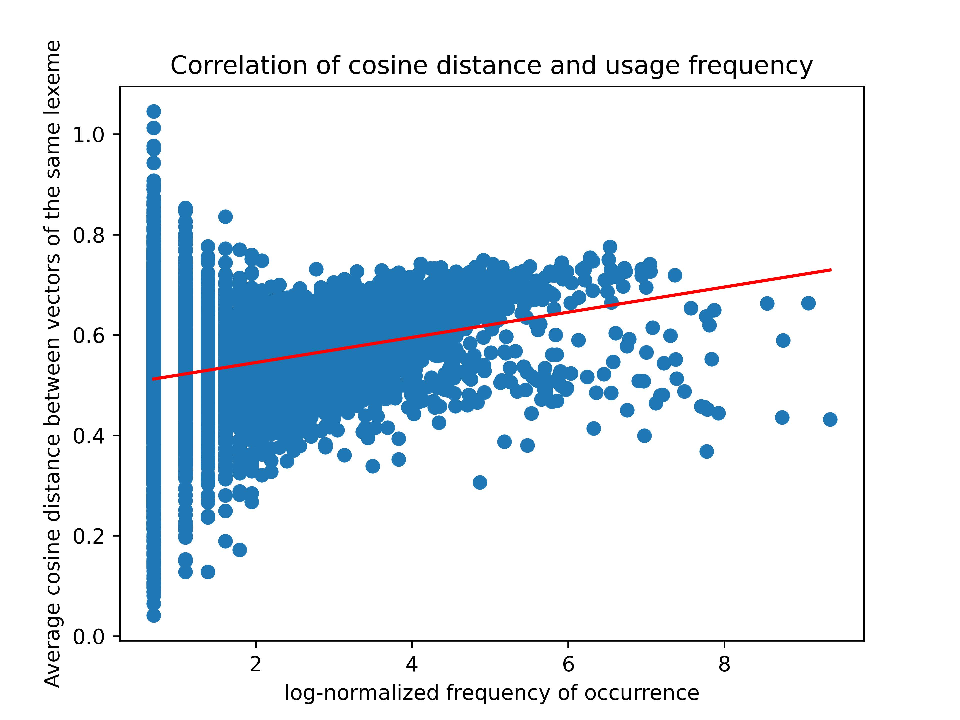
\includegraphics[width=\linewidth]{cos_dist_vs_freq}
	\caption{Correlation of average cosine distance and frequency of occurrence. Each blue dot represents the average cosine distance between all vectors for one lemma. Each vector was computed from one usage context of the lemma in the corpus. The red line indicates a linear regression of average cosine distance and usage frequency.}
	\label{figure:cosineDistanceVsFrequency}
\end{figure}
The second observation may serve as a reminder that we have to be particularly cautious when looking at low-frequency lemmata: Their relatively high variance in average cosine distance indicates a widely varying degree of polysemy. We can validate our operationalization of polysemy through cosine distance by manually inspecting conspicuous cases: Lemmata that occur twice in the whole corpus and only within the same sentence are, by definition, the least polysemous in our setting. The reasons for this behavior are as follows:
\begin{itemize}
	\item Hapax Legomena have been discarded from the inspection because they only have one vector and cosine distance is not easily applicable to anything but pairs of vectors.
	\item The vectors are computed using distributional information (i.e. which other words appear in the sentence) and positional encoding. If a lemma appears twice in a sentence, the vectors for the two instances will differ mainly in their positional encoding, but not so much in the distributional information. This leads to very similar vectors with a low cosine distance.
\end{itemize}
Therefore, lemmata with 2 occurrences that both stem from the same sentence (e.g. \textit{Augustofratensis, Constantinopolis} or \textit{Sychem}, found in PROIEL 57662, 57780 and 23738, respectively) are prime examples for a low degree of polysemy. The phenomenon of low-frequency words tending to appear multiple times in quick succession (instead of a smooth distribution over the whole corpus) is referrd to as burstiness. It often results from a topical focus, which in turn influences lexis \parencite[99]{pierrehumbertBurstinessVerbsDerived2012}. This is also true for PROIEL, as we can quickly determine from a simple calculation: 1,271 lemmata are Dis Legomena, i.e. they occur exactly twice in the corpus. 37 of them occur only within a single sentence. Thus, the observed probability of encountering both instances of a Dis Legomenon in a specific sentence is 37 / 19,335 = 0.002 , where 19,335 is the total number of sentences in the corpus. If, on the other hand, we take up a theoretical position and naively expect an equal probability of occurrence for Dis Legomena in each sentence, our expectation would look like this:
\begin{itemize}
	\item In the whole corpus, there are 19,335 sentences with 217,797 tokens, which in turn derive from 8,872 lemmata.
	\item On average, each sentence contains about 11 tokens. Each of them could belong to any lemma. The probability of meeting an instance of a specific lemma at a specific place in the sentence is 1 / 8,872 = 0.0001 . An average sentence could be modeled as a sequence of Bernoulli trials, where the chance of success (i.e. meeting a specific lemma) at each token is 0.0001 . The chance of meeting that same lemma exactly twice in a sentence is then \( P(k) = \binom{n}{k} \times p^k \times q^{n-k} \), where \textit{n} is the number of trials, \textit{k} is the desired number of successes, \textit{p} is the probability of success and \textit{q} the one of failure.
	\item Thus, \( P(k) = \binom{11}{2} \times 0.0001^2 \times 0.9999^{11-2} = 55 \times 0.00000001 \times  0.9991 = 0.0000005 \). Since we want to exclude any lemmata that are not Dis Legomena, we have to divide that result by a factor that corresponds to the fraction of Dis Legomena compared to all lemmata, i.e. 1,271 / 8,872 = 0.14 . As a consequence, our theoretical chance of encountering both instances of a Dis Legomenon in the same sentence becomes even smaller (0.00000007).
\end{itemize}

Now, we can compare that theoretical value (0.00000007) to the actually observed probability of encountering both instances of a Dis Legomenon within the same sentence (0.002), which is almost 30,000 times higher. This immense deviation from our expectations leads to the conclusion that Bernoulli Trials are not a good model for lexis in sentences of this Latin corpus. We may even go further and argue that many statistical measures cannot be reasonably applied to language corpora because their mathematical preconditions are not met by the data \parencite[110]{shadrovaMeasuringCoselectionalConstraint2020}. In particular, the words in a corpus are not distributed equally and their relative frequencies do not converge after a certain amount of time \parencite[5]{debowskiNaturalLanguagePerigraphic2018}.

%TODO: Alternativen zu TTR für lexikalische Dichte?
The \hyperref[firstObservation]{first observation}, on the other hand, suggests a positive correlation between polysemy and usage frequency: Words that we use more frequently tend to be more flexible in their meaning from a distributional point of view \parencite[576]{crossleyDevelopmentPolysemyFrequency2010}. We can verify that claim by subsampling a specific amount of usage contexts for every type in the corpus and calculating the \gls{TTR} \parencites[229]{kettunenCanTypetokenRatio2014}[1]{hamiltonDiachronicWordEmbeddings2016} for them:

\begin{enumerate}
	\item Select all types from PROIEL with an occurrence frequency $\geq$10.
	\item For every selected type, collect all tokens that occurred in the same sentences as that type.
	\item Omit all types did not occur together with at least 100 tokens.
	\item For the remaining types, randomly sample 100 tokens from their usage contexts.
	\item From the selected tokens, calculate the \gls{TTR} for each type.
\end{enumerate}

The thresholds of 10 and 100 were arbitrarily chosen. Their main purpose is to ensure that we have enough (i.e., 10) instances of a single type to avoid the large variance that became apparent in Fig. \ref{figure:cosineDistanceVsFrequency} and to mitigate the influence of text length effects (max. 100 tokens per type), which is a known problem for \gls{TTR} and other measures of lexical diversity \parencite[66]{koizumiRelationshipsTextLength2012}. Nevertheless, in the lower left corner of Fig. \ref{figure:ttr_vs_frequency} (\gls{TTR} <0.6, frequency <4), we can still observe some traces of higher lexical variance in low-frequency types. Generally, as indicated by the linear regression, high-frequency types tend to exhibit a slightly larger lexical diversity in their usage contexts. This underlines the importance of explicitly dealing with issues of polysemy in the extraction of hyponyms for language learning, as was \hyperref[high_frequency_hyponyms_for_language_learning]{outlined above}.

\begin{figure}[ht]
	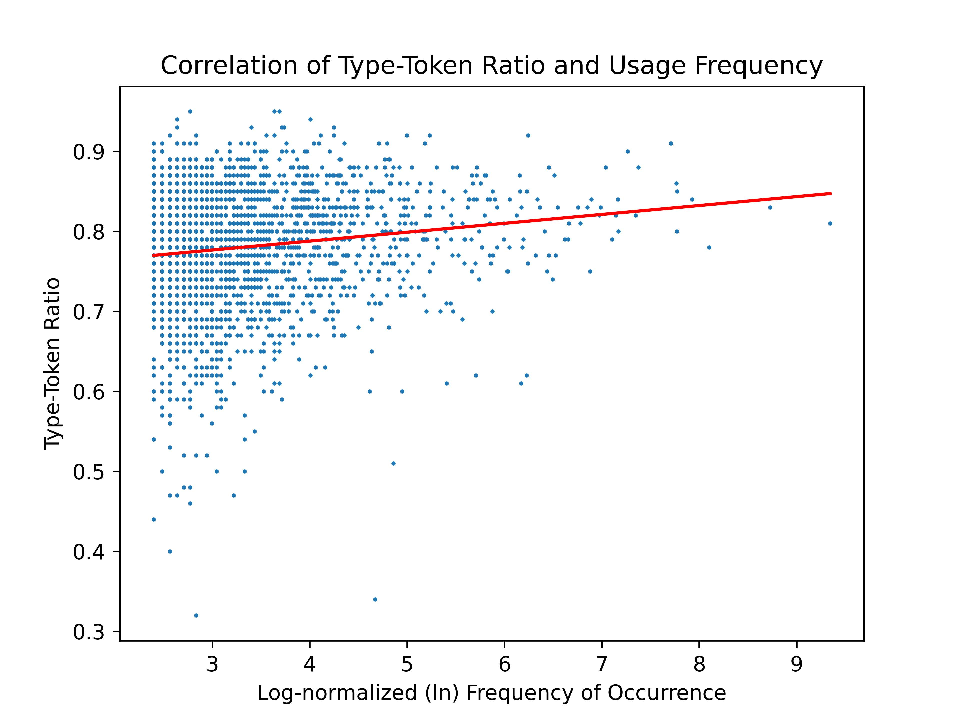
\includegraphics[width=\linewidth]{ttr_vs_freq.pdf}
	\caption{Correlation of \gls{TTR} and frequency of occurrence. Each blue dot represents a specific type. \gls{TTR}s were calculated only for types that occur at least 10 times in the corpus and have at least 100 tokens in their aggregated usage contexts, i.e., sentences. For the chosen types, a random sample of 100 tokens was selected for the calculation of \gls{TTR} to avoid text length effects. The red line represents a linear regression.}
	\label{figure:ttr_vs_frequency}
\end{figure}

\section{Clustering of Contextual Embeddings}
As we outlined before, the actual clustering of usage contexts for every token in the PROIEL corpus will be performed on the lexeme level. The procedure is as follows:
\begin{enumerate}
	\item For every token in the corpus, compute its embedding vector in the sentence context.
	\item Initially, treat every embedding vector as its own cluster.
	\item For every pair of clusters, compute the similarity between their vectors. If a cluster contains more than one vector, compute the average for all of its vectors and use that for comparison to the other cluster.
	\item Merge those clusters that are very close to each other.
	\item Repeat steps 3 and 4 until a specific threshold is reached.
\end{enumerate}

Ideally, the recursive iterations should take place after every merging of two clusters. This way, the newly formed cluster has a chance to be merged again immediately (if its similarity to another cluster is still above the threshold). However, for computational reasons, we instead use small batches of 15 clusters and compute the similarity values between all distinct pairs for them. This leads to about 15,000 batches being simultaneously processed in every iteration. Thus, the clustering method loses some of its accuracy while being substantially faster to compute.

The initial number of clusters, where each usage context represents its own cluster, is 217,923 , which corresponds closely to the number of tokens in the PROIEL corpus (217,797). 
%TODO: explain the difference (126 or 0.06%) between usage contexts / clusters and PROIEL tokens
By using a threshold of 0.9 for the cosine similarity that is required to merge two clusters, exactly 1 new cluster emerges. Correspondingly, the overwhelming majority of clusters was not merged at all. The merged cluster contains two usage contexts of the word \textit{et} `and':

\vspace{10pt}
\ex[exno=PROIEL 11203]
	\begingl
		\gla et responde-ns Iesus ai-t ill-is //
		\glb and reply-{\sc part.pres} Jesus say.{\sc impf-3sg} that-{\sc pl.dat/abl} //
		\glft and Jesus replied to them by saying //
	\endgl
\xe 
\vspace{10pt}
\ex[exno=PROIEL 16513]
	\begingl
		\gla et responde-ns Iesus ai-t ill-i //
		\glb and reply-{\sc part.pres} Jesus say.{\sc impf-3sg} that-{\sc dat} //
		\glft and Jesus replied to him by saying //
	\endgl
\xe
\vspace{10pt}

The two sentences differ only in their lexis, and only in the last token. Even for those last tokens, the relevant lemma (\textit{ille} `he, that') is the same. Thus, the representations are so close to each other (cf. Table \ref{tableCosSimWordSubstitution}) that they get merged into a larger cluster quite easily.

This changes when we set the similarity threshold to 0.8 . To achieve a higher performance of the clustering algorithm, we do not perform this additional processing step on the original clusters that were all unmerged. Instead, we use the results of the first clustering phase, which is not important in this early phase (because it barely differs from the original clusters), but will be crucial later on. This procedure yields 41 merged clusters, some of which contain up to 4 usage contexts. All in all, the merged vectors now include 88 (0.04\%) usage contexts. Interestingly, the merges occurred not just for further instances of \textit{et} `and' (e.g., PROIEL 10565 and 48782) or other function words like \textit{ibi} `there' (PROIEL 57777 and 78440), but also for seemingly unrelated pairs like \textit{videam -- diligentiam} `I may see -- carefulness': 

\vspace{10pt}
\ex[exno=PROIEL 77240]
	\par
	\begingl
		\gla itaque exspect-o Thessalonic-ae act-a Kal Sext ex qu-ibus statu-a-m in tu-os ne agr-os confugi-a-m ut ne que vide-a-m homin-es qu-os nol-i-m et te ut scrib-is vide-a-m et prop-ius si-m si quid ag-a-tur id que intelle-x-i cum t-ibi tum Quint-o fratr-i placere an abe-a-m Cyzic-um //
		\glb thus wait-{\sc 1sg} Thessaloniki-{\sc loc} transaction-{\sc pl} first.day august from which-{\sc pl.abl} decide-{\sc sbjv-1sg} into your-{\sc pl.acc.m} whether field-{\sc acc.pl} flee-{\sc sbjv-1sg} so.that not =and see-{\sc sbjv-1sg} man-{\sc pl} who-{\sc pl.acc.m} be.unwilling-{\sc sbjv-1sg} and you.{\sc acc} as write-{\sc 2sg} see-{\sc sbjv-1sg} and near-{\sc comp} be.{\sc sbjv-1sg} if something conduct-{\sc sbjv-3sg.pass} this.{\sc n} =and  perceive-{\sc perf-1sg} when you-{\sc dat} then Quintus-{\sc dat/abl} brother-{\sc dat} please or go.away-{\sc sbjv-1sg} Cyzicus-{\sc acc} //
		\glft Thus, I wait at Thessaloniki for the transactions of August 1. On the basis of them, I will decide whether to take refuge at your estate, so that I may not have to see those that I do not want to, and instead see you (as you wrote to me), and be closer if anything happens (and this, I have learned, is pleasant for you and especially for Quintus), or to go away to Cyzicus //
	\endgl
\xe 
\vspace{10pt}

\ex[exno=PROIEL 77314]
	\par
	\begingl
		\gla in qu-o si iam nostr-a salus cum hac leg-e despera-t-a eri-t vel-i-m pro tu-o in me amor-e hanc inan-em me-am diligentia-m miserabil-em potius quam inept-am put-e-s sin es-t aliquid spe-i d-e-s opera-m ut ma-ior-e diligenti-a posthac a nostr-is magistrat-ibus defend-a-mur //
		\glb in which-{\sc abl.n/m} if already our-{\sc f} salvation with this.{\sc f.abl} law-{\sc abl} give.up-{\sc part.perf.pass-f.sg/n.pl} be.{\sc fut-3sg} want-{\sc sbjv-1sg} for.the.sake.of your-{\sc dat/abl.m/n} towards I.{\sc acc} love-{\sc abl} this.{\sc f.acc} useless-{\sc acc.m/f} my-{\sc f.acc} diligence-{\sc acc} pitiful-{\sc acc.m/f} rather than silly-{\sc f.acc} think-{\sc sbjv-2sg} if.however be-{\sc 3sg} anything hope-{\sc gen/dat} give-{\sc sbjv-2sg} effort-{\sc acc} so.that large-{\sc comp-abl} diligence henceforth by our-{\sc pl.dat/abl} official-{\sc pl.dat/abl} defend-{\sc sbjv-1pl.pass} //
		\glft Regarding this matter, if my salvation will already be hopeless together with this law, I would like you to think, because of your love towards me, that my useless diligence is pitiful rather than silly; if, however, there is any kind of hope, please try to make sure that, in the future, we will be defended by our officials with greater diligence //
	\endgl
\xe
\vspace{10pt}

The passages belong to Cicero's Letter to Atticus, book 3, letters 15 and 23. They share almost no vocabulary except for function words like \textit{tuus} `your', \textit{ut} `that, so that', or \textit{si} `if'. Their semantic similarity is possibly related to the overlap of involved persons (Cicero and Atticus), but Cicero's brother Quintus is mentioned in the first passage. Another factor is the narrative structure: both passages outline two potential future scenarios. In the first letter, Cicero ponders on his next action:
\begin{enumerate}[label=(\alph*)]
	\item go to Atticus' estate
	\item go to Cyzicus
\end{enumerate}
Correspondingly, the second letter shows two potential outcomes that Cicero wishes for:
\begin{enumerate}[label=(\alph*)]
	\item Atticus should feel pity for him (if all hope is relinquished)
	\item Atticus should get the officials on Cicero's side (if he gets the chance)
\end{enumerate}



%TODO: FIX THIS
The distribution of cluster size seems to follow a Zipfian distribution (see Fig. \ref{figure:cluster_size_distribution}). 

\begin{figure}[ht]
	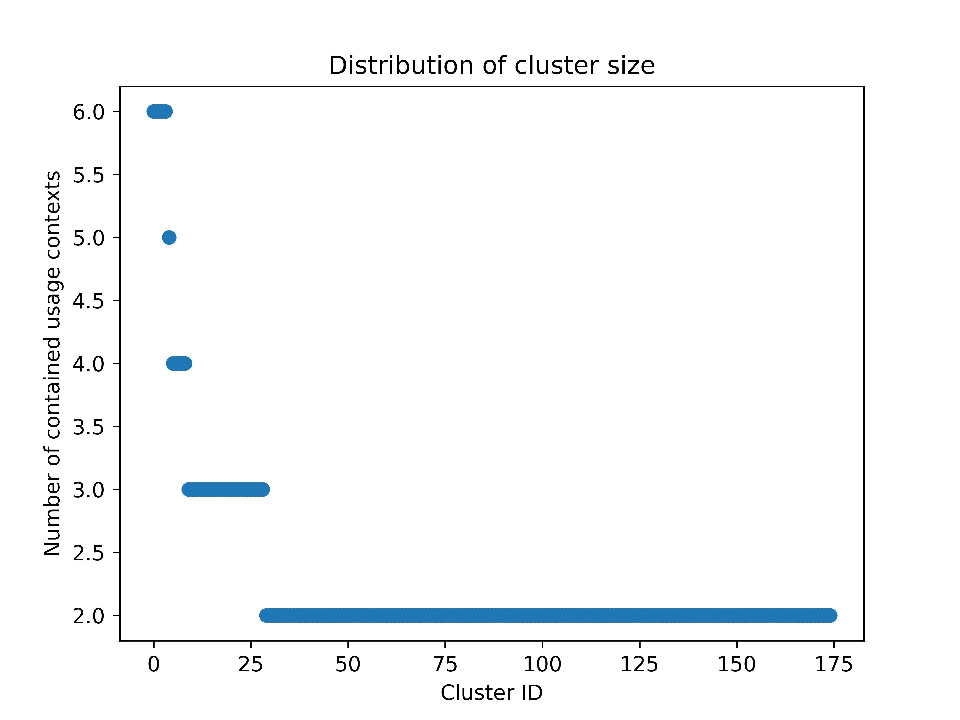
\includegraphics[width=\linewidth]{cluster_size_distribution.pdf}
	\caption{Distribution of cluster size for merged clusters at a similarity threshold of 0.9 . The largest cluster (128 usage contexts) was excluded for better legibility.}
	\label{figure:cluster_size_distribution}
\end{figure}

All merged clusters consist of usage contexts for the same lemma, i.e., there are no cross-lexeme clusters. This does not change if we lower the similarity threshold to 0.8, 

%TODO: mbert demo, document-level domain embeddings, glossing; explain custom glosses?

%As for the gold standard on hyponymy, the Latin part of the WordNet was used. In a very basic approach, we will extract from it the explicit hyponym and hypernym pairs only for nouns, converting both to the notation of "hyponym,hypernym". This ignores additional properties like transitivity in order to create an explicit empirical baseline for later comparison. Besides, since there is no previous empirical knowledge from applying machine learning to hyponymy detection in Latin, we shall transform the complex problem to a much simpler one and then, gradually, reintroduce the complexity: At the very beginning, the machine's task will be to detect whether there are instances of hyponymy in a given sentence or not, which is called binary classification because there are only two options (either there are some instances or there are none). Eventually, the most complex question may look something like this: Given a Latin text passage, which words in it are hyponyms of which other ones and which word sense do they express in that specific context? Notably, the main dimensions of complexity are the following:
%\begin{itemize}
   %      \item The input can be a sentence (easy) or some longer kind of segment, e.g. a paragraph (difficult).
      %   \item The detection can be binary (easy) or token-based (difficult).
         %\item Polysemy can be leveled (easy) or explicitly disambiguated (difficult).
%\end{itemize}
%Furthermore, there are various ways of balancing to consider. By comparing plain text to the WordNet lemmata in a superficial manner, we can only detect hyponymy for those sentences in which the hyponyms appear in their base form. For languages with little inflectional variety (like English), this may be an acceptable choice. For Latin, however, with its rich morphology, such a simplification has far-reaching consequences: About 3\% of the sentences were associated with hyponymy (see Table ~\ref{table:hyponymyPercentageShallow}).

%\begin{table}[ht]
%	\begin{tabular}{ c | c | c }
  %		 & All Sentences & With Hyponyms \\ \hline
  %		Absolute & 9 992 000 & 304 677 \\
  %		Percentage & 100\% & 3.05\%  \\
	%\end{tabular}
	%\caption{Percentage of sentences with hyponymy, extracted by shallow comparison to WordNet}
	%\label{table:hyponymyPercentageShallow}
%\end{table}

%Therefore, machines will achieve high accuracy rates (>95\%) using rather simple rules, e.g. by never predicting a hyponym. Alternatively, they may produce similar results by memorizing all of the (most frequent) hyponyms: There are 6781 noun lemmata in WordNet that also appear as surface forms in the Corpus Corporum. As with many linguistic frequency distributions, their occurrence counts follow Zipf's law \parencite[VI]{zipfPsychobiologyLanguageIntroduction1936}. In other words, a few "super-hypernyms" like \textit{causa} (cause, reason), \textit{genus} (race, kind) or \textit{homo} (human being, man) dominate the overall picture, leaving rarely occurring nouns such as  \textit{concussio} (shaking, concussion),  \textit{audientia} (hearing, listening) or  \textit{congelatio} (freezing, congealing) far behind. This information will be helpful for language learning purposes because, in some cases, rather superordinate terms may be acquired later than their prototypical hyponyms \parencite[27]{ellisUsagebasedLanguageInvestigating2013}. This is true for the acquisition of both L1 and L2. In Latin, however, we are not concerned with acquisition, but with learning: Students usually do not speak Latin in their everyday life or during  classes, except when occasionally reading aloud a text. Reciting Latin texts does not (yet) seem to be a well-defined concept in terms of language learning \parencite[243, fn. 89]{munznerNeueWegeIm2013}.

%(see Table ~\ref{table:modelAccuracyShallow})
%\begin{table}[ht]
%	\begin{tabular}{ c | c | c | c }
  %		 & Precision & Recall & F1 \\ \hline
  %		Score & .73 & .41 & .53 \\
	%\end{tabular}
	%\caption{Evaluation of the simplest model, trained with data from a shallow comparison to WordNet}
	%\label{table:modelAccuracyShallow}
%\end{table}
%\begin{figure}[ht]
%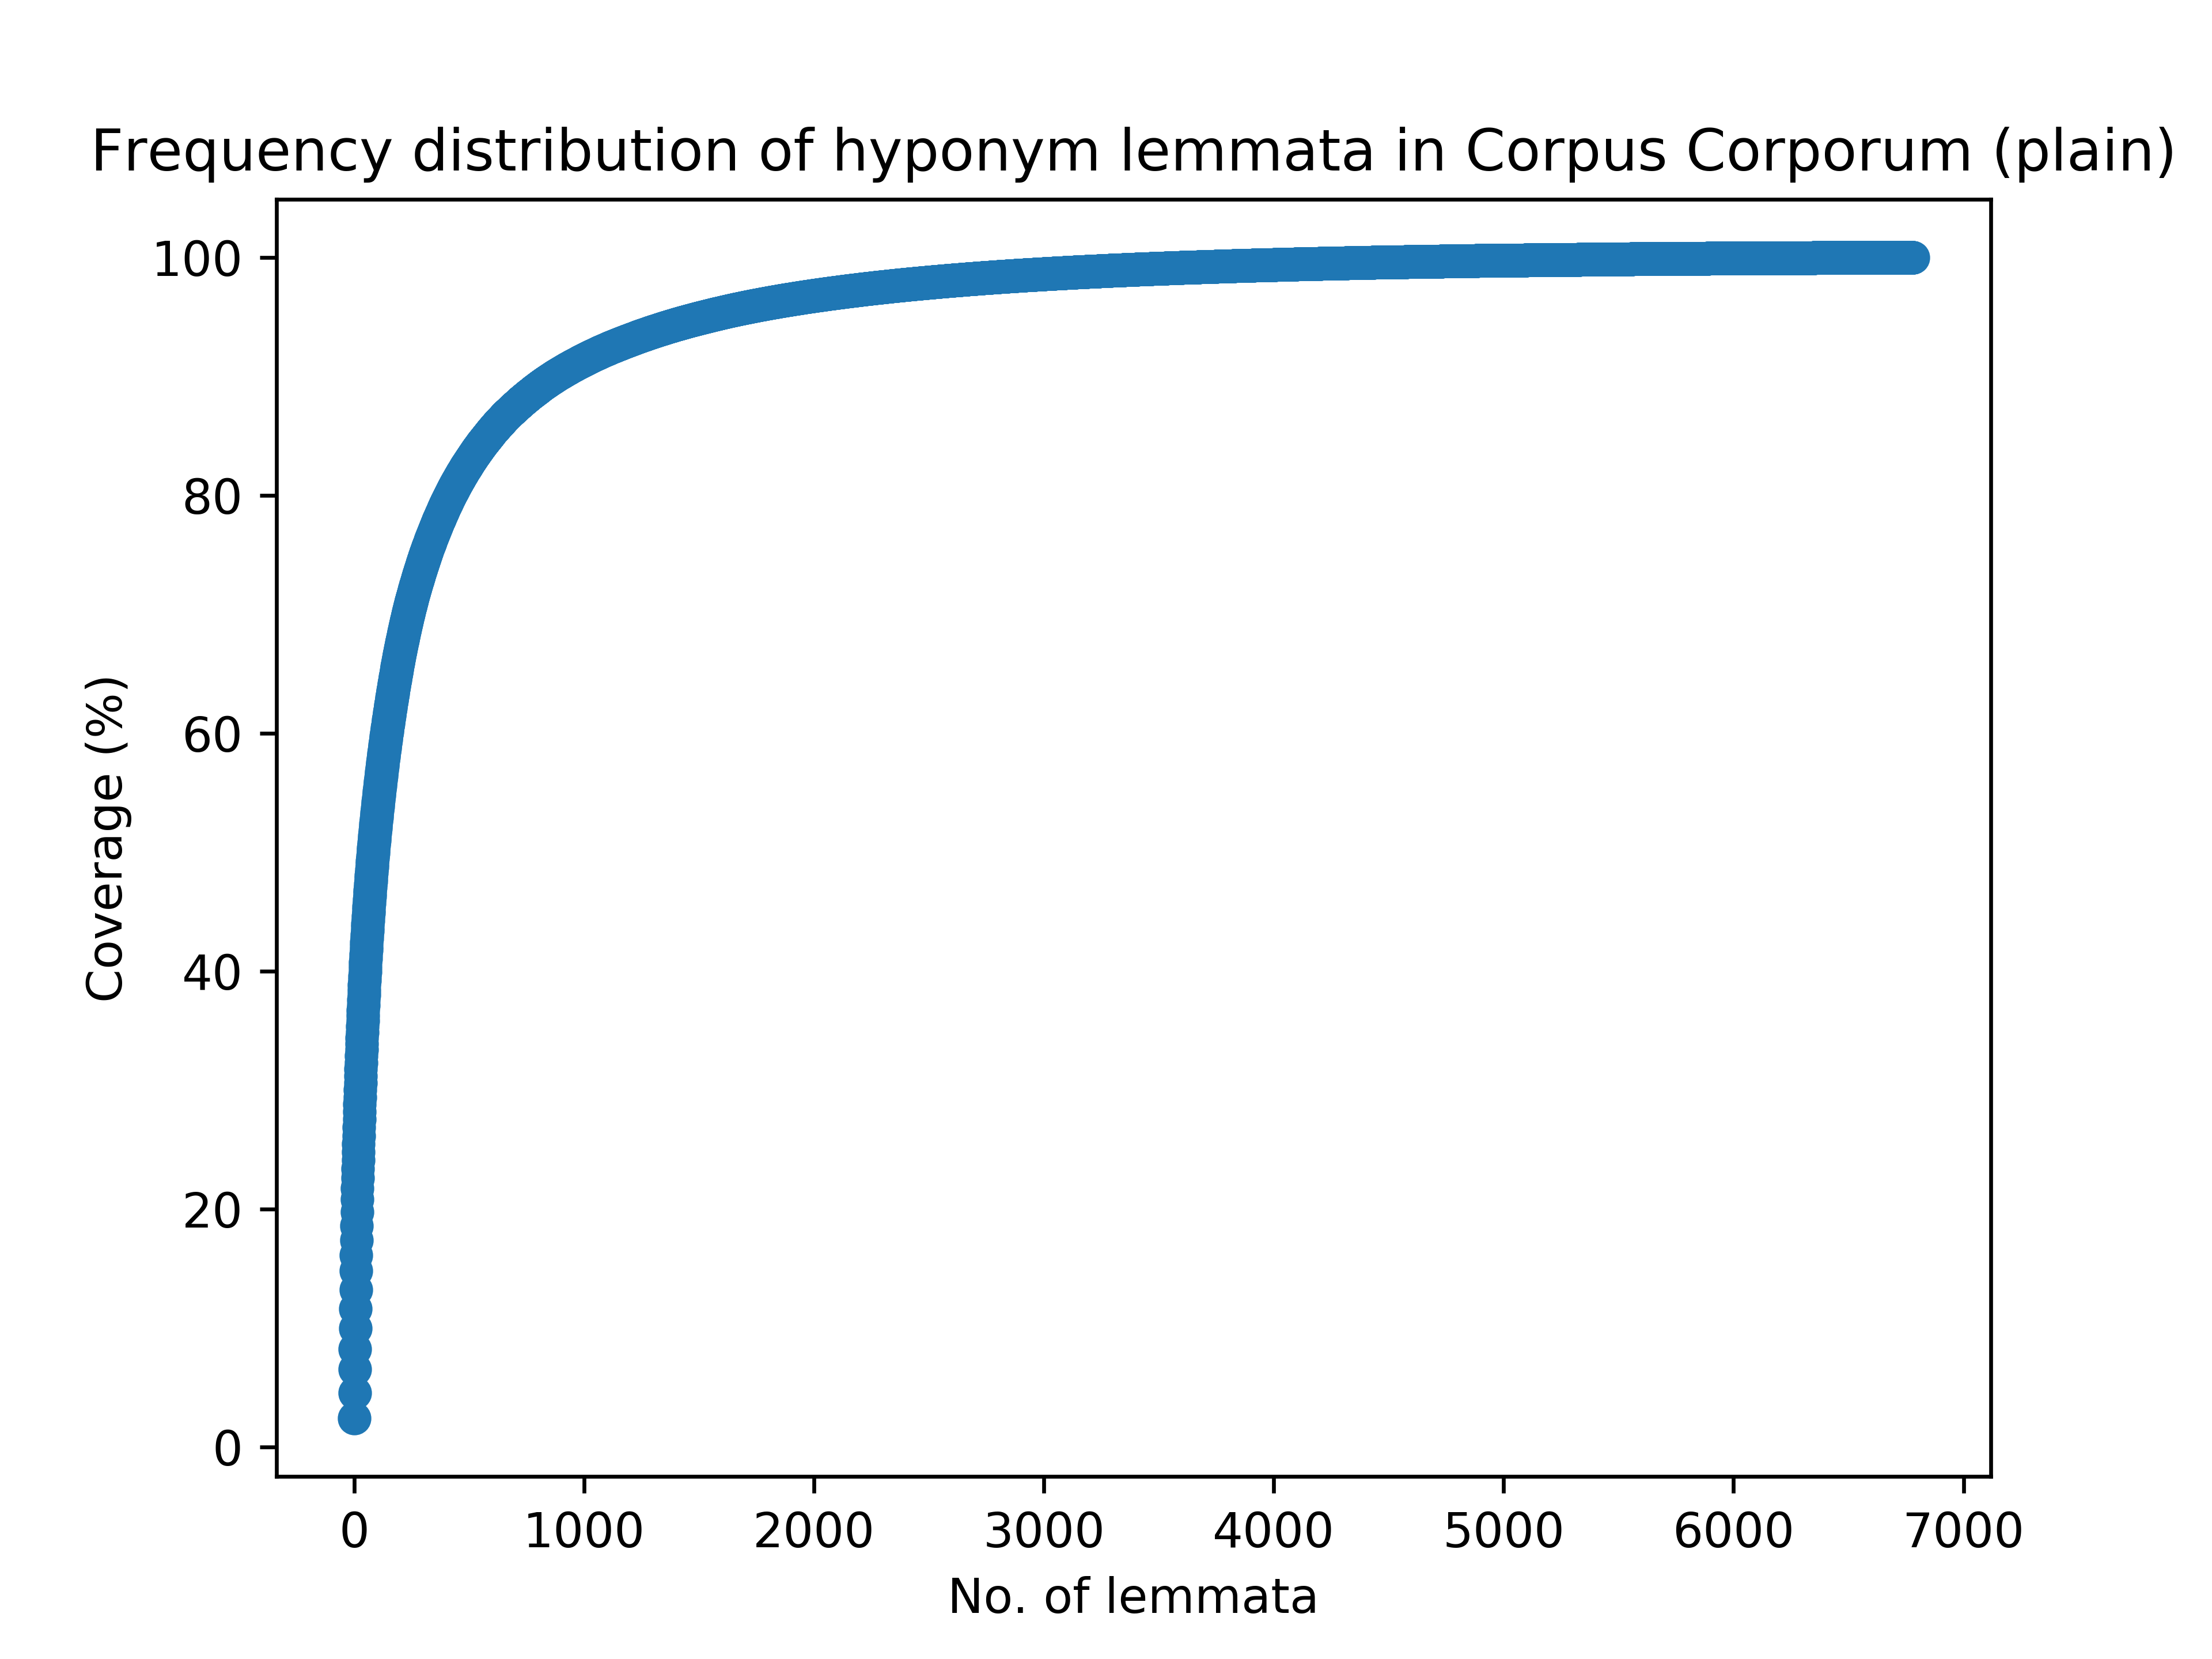
\includegraphics[width=\linewidth]{freq_dist_hyponyms_cc_plain}
%\caption{Frequency distribution of hyponym lemmata in the Corpus Corporum (plain text)}
%\label{figure:frequencyDistributionHyponymsCCplain}
%\end{figure}

\chapter{Appendix}
\section{Appendix A: Agile and Open Methodology}
\label{sec:appendixA}
This study will follow an approach which is borrowed from computer science, namely the agile methodology for software development \parencite[32]{fowlerAgileManifesto2001}. Coding will be used to establish a proof of concept for this study by implementing the discussed models and testing them on real-world corpus data. Furthermore, the basic notion of incremental and iterative progress also applies to the way the models themselves are being created: The dissertation will see a range of approaches and considerations being applied for various purposes, which reflects my own thoughts about the detection of semantic relations growing from initial, very basic foundations (e.g. plain contingency tables) to more complex environments of semantic study. The application of agile methodology to linguistic research is motivated not just by the related coding activities, but also by the similarities between dissertations and software products: In this view, a dissertation can be seen as a product to be delivered to customers, i.e. the research community. The analogy is enhanced further by the overlapping quality factor of openness: Dissertations are necessarily products of open science in much the same way as open source software is the product of other communities sharing the desire for unrestricted public access to creative commons \parencite[518]{garcia-penalvoOpenKnowledgeManagement2010}. 

To demonstrate the viability of this transfer, the dissertation is split into various modules, separating, e.g., the bibliography from the rest of the documents and employing cross-references to put it all together for presentational purposes. These modules are, to some extent, directly visible in the sense of multiple source files that may be compiled to form a more complex document. Also, they are all publicly accessible at \href{https://github.com/konstantinschulz/asrael} and subject to version control, thus enabling readers to trace the resulting thoughts back to their very roots. Eventually, the reason to make all these considerations explicit is not so much to suggest a high quality of the work process, but rather to emphasize their possibly tremendous influence on the results and how they are gathered.

\printbibliography[heading=bibintoc]

\end{document}
























